% Author: Santiago Faci <santiago.faci@gmail.com>
% www.videosdeinformatica.com

\documentclass[xcolor={dvipsnames}]{beamer}
\setbeamertemplate{navigation symbols}{}

\usepackage{beamerthemeshadow}
\usepackage[spanish]{babel}
\usepackage{url}
\usepackage[utf8]{inputenc}

\definecolor{resalta}{cmyk}{0,1,0,0}

\usepackage{listings}
\lstset{basicstyle=\tiny\ttfamily,breaklines=true}
\lstset{framextopmargin=50pt}
\lstset{keywordstyle=\tiny\color{blue}\bfseries}
\lstset{stringstyle=\tiny\color{red}\ttfamily}
\lstset{commentstyle=\tiny\color{OliveGreen}\ttfamily}
\lstset{showstringspaces=false}

\begin{document}
\title{Programación Multimedia y Dispositivos Móviles: Desarrollo de Videojuegos con libGDX}
\author{Santiago Faci}
\institute{}
\date{} 

\begin{frame}
\titlepage
\end{frame}

\begin{frame}[plain]\frametitle{Índice}\tableofcontents
\end{frame} 


\section{¿Qué es libGDX?} 
\begin{frame}\frametitle{¿Qué es libGDX?} 
    \begin{block}{libGDX}
    \begin{itemize}
        \item \emph{\textcolor{resalta}{libGDX}} es un framework multiplataforma para el desarrollo de videojuegos en lenguaje Java. A este tipo de frameworks también se les conoce como \emph{motores de videojuegos (game engine)}
        \item Permite desarrollar videojuegos para Desktop (Windows, Linux, MacOS X), iOS, Android, BlackBerry y HTML5
        \item Se integra con los IDEs más conocidos (IntelliJ IDEA, eclipse, NetBeans)
        \item Dispone de APIs de alto nivel para 2D y 3D
        \item Incorpora motor de físicas (\emph{\textcolor{resalta}{Box2D}})
    \end{itemize}
    \end{block}
\end{frame}

\begin{frame}\frametitle{¿Qué es libGDX? (más)}
	\begin{block}{libGDX}
    \begin{itemize}
		\item Tiene una librería propia para trabajar con \emph{TiledMaps}
		\item Buena documentación y comunidad de desarrolladores (muy en auge últimamente)
		\item Desarrollo en activo \href{http://libgdx.badlogicgames.com}{\beamerbutton{Página web}}
    \end{itemize}
    \end{block}
\end{frame}

\subsection{Conceptos de videojuegos}
\begin{frame}\frametitle{Algunas definiciones}
	\begin{block}{Frame}
		Cada uno de los fotogramas que se visualizan en pantalla en un videojuego
	\end{block}
	\begin{block}{Renderizar}
		Dibujar en pantalla algún elemento de un videojuego
	\end{block}
	\begin{block}{FPS (Frames Per Second)}
		Número de frames por segundo que un juego es capaz de renderizar. 30 FPS proporcionan una jugabilidad fluida
	\end{block}
\end{frame}

\begin{frame}\frametitle{Algunas definiciones (más)}
	\begin{block}{Textura}
		Cada una de las imágenes 2D cargadas en memoria para usar en un videojuego
	\end{block}
	\begin{block}{Sprite}
		Representa una textura junto con su posición \emph{x} e \emph{y} en la pantalla
	\end{block}
	\begin{block}{Animación (2D)}
		Conjunto de texturas 2D en movimiento en un videojuego. Hay que tener en cuenta que un instante determinado solamente se verá en
        pantalla una textura determinada
	\end{block}
\end{frame}

\begin{frame}\frametitle{Algunas definiciones (y más)}
	\begin{block}{Texture Atlas}
		Conjunto de texturas almacenadas en un mismo fichero. Reduce el tiempo de carga puesto que en un solo acceso a disco se pueden
        cargar todas las texturas de un videojuego
	\end{block}
	\begin{block}{Delta Time (dt)}
		Tiempo que necesita el ordenador para procesar cada uno de los frames de un videojuego, medido en segundos (normalmente son valores 
        muy cercanos a cero)
	\end{block}
\end{frame}

\section{Estructura de libGDX} 
\subsection{Estructura de módulos}
\begin{frame}\frametitle{Estructura de módulos}
    \begin{figure}
    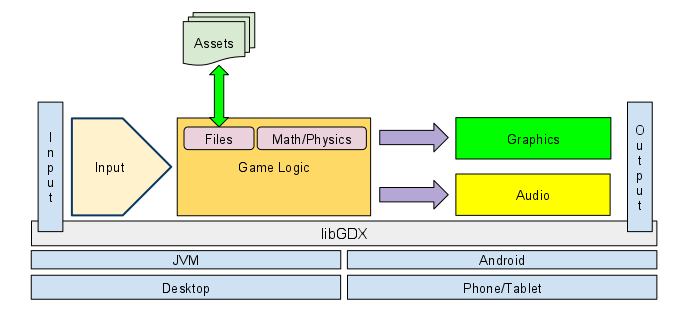
\includegraphics[scale=0.4]{images/modules_overview} 
    \caption{Framework libGDX}
    \end{figure}
\end{frame}

\subsection{Ciclo de vida de un videojuego}
\begin{frame}[plain]\frametitle{Ciclo de vida de un videojuego}
    \begin{figure}
    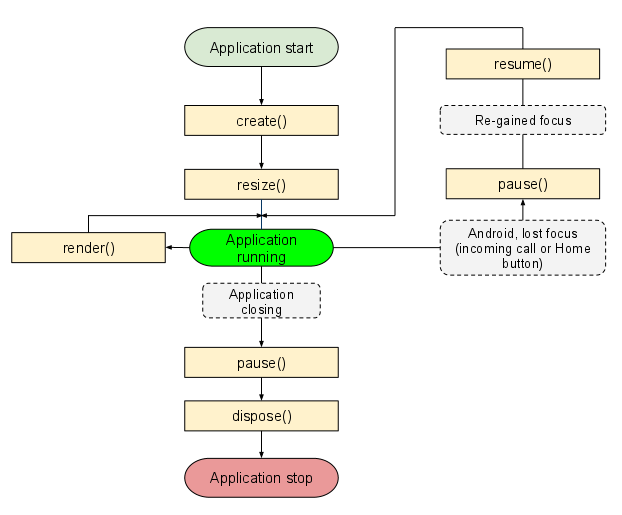
\includegraphics[scale=0.4]{images/libgdx_lifecycle} 
    \caption{Ciclo de vida de un videojuego desarrollado con libGDX}
    \end{figure}
\end{frame}

\subsection{Estructura de un videojuego}
\begin{frame}\frametitle{Estructura de un videojuego}
    \begin{columns}
        \begin{column}{4cm}
        \begin{figure}
        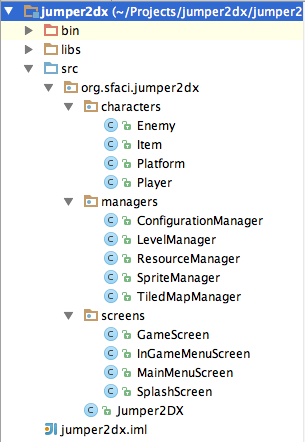
\includegraphics[scale=0.3]{images/project_structure} 
        \caption{Proyectos videojuego libGDX}
        \end{figure}
        \end{column}
        \pause
        \begin{column}{6cm}
        \begin{block}{}
        \begin{itemize}
            \item \emph{\textcolor{resalta}{jumper2dx}} Proyecto principal
            \item \emph{\textcolor{resalta}{jumper2dx-desktop}} Proyecto Escritorio
            \item \emph{\textcolor{resalta}{jumper2dx-android}} Proyecto Android
            \item \emph{\textcolor{resalta}{jumper2dx-html5}} Proyecto HTML5
            \item \emph{\textcolor{resalta}{libs}} Librerias libGDX
            \item \emph{\textcolor{resalta}{assets}} Recursos
            \item \emph{\textcolor{resalta}{src}} Código del videojuego
        \end{itemize}
        \end{block}
        \end{column}
    \end{columns}
\end{frame}

\begin{frame}\frametitle{Proyecto Principal}
	\begin{itemize}
		\item Se incluye toda la programación del videojuego, puesto que será común aunque se desarrolle para más de una plataforma diferente
		\item Se desarrolla como un proyecto diferente de la aplicación
		\item No incluye ninguna clase con un método \emph{main()}, puesto que necesita de algún proyecto lanzadera para ejecutarse
		\item Debido al funcionamiento de \emph{\textcolor{resalta}{libGDX}}, los \emph{assets} del videojuego se deben incluir en uno de los proyectos lanzadera y enlazarlos desde el resto de proyectos
	\end{itemize}
\end{frame}

\begin{frame}[plain]\frametitle{Proyecto Principal: estructura de clases}
	\begin{block}{}
	\begin{itemize}
		\item characters
		\begin{itemize}
			\item \emph{\textcolor{resalta}{Character1}}
			\item \emph{\textcolor{resalta}{Character2}}
			\item . . .
		\end{itemize}
		\item screens
		\begin{itemize}
			\item \emph{\textcolor{resalta}{MainMenuScreen}} Pantalla de inicio del videojuego
			\item \emph{\textcolor{resalta}{GameScreen}} Pantalla de juego
			\item \emph{\textcolor{resalta}{GameOverScreen}} Pantalla de fin de partida
		\end{itemize}
		\item managers
		\begin{itemize}
			\item \emph{\textcolor{resalta}{ResourceManager}} Gestiona los recursos (\emph{assets}) del videojuego
			\item \emph{\textcolor{resalta}{SpriteManager}} Gestiona la lógica del videojuego
			\item \emph{\textcolor{resalta}{LevelManager}} Gestiona los niveles (y el paso entre éstos) del videojuego
			\item \emph{\textcolor{resalta}{ConfigurationManager}} Gestiona la configuración del juego (\emph{settings})
		\end{itemize}
		\item utils
		\begin{itemize}
			\item \emph{\textcolor{resalta}{Constants}} Clase de constantes de aplicación
			\item \emph{\textcolor{resalta}{Util}} Clase de métodos de utilidad (\emph{Helpers})
		\end{itemize}
	\end{itemize}
	\end{block}
\end{frame}

\begin{frame}\frametitle{Estados de un videojuego}
    \begin{block}{}
    \begin{figure}
    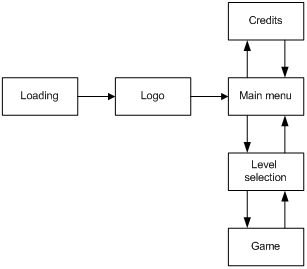
\includegraphics[scale=0.5]{images/game_screens} 
    \caption{Estados de un videojuego}
    \end{figure}
    \end{block}
\end{frame}

\begin{frame}\frametitle{Estados de un videojuego (II)}
    \begin{block}{}
    \textcolor{resalta}{libGDX} proporciona las clases \textcolor{resalta}{Game} y \textcolor{resalta}{Screen} para poder implementar los
    estados de nuestro juego:
    \begin{itemize}
        \item La clase \textcolor{resalta}{Game} permite cargar el juego y realizar la transición entre los diferentes estados (\emph{Screens}) del mismo
        mediante los métodos \textcolor{resalta}{setScreen()} y \textcolor{resalta}{getScreen()} que permiten, respectivamente, pasar a otro
        estado del juego y obtener el estado actual del juego.
        \item La interfaz \textcolor{resalta}{Screen} proporciona el ciclo de vida completo de un videojuego a cada uno de los estados del
        mismo (métodos \textcolor{resalta}{show()}, \textcolor{resalta}{render()}, \textcolor{resalta}{resize()},
        \textcolor{resalta}{hide()}, \textcolor{resalta}{pause()}, \textcolor{resalta}{resume()} y \textcolor{resalta}{dispose()})
    \end{itemize}
    \end{block}
\end{frame}

\begin{frame}\frametitle{Managers}
	\begin{itemize}
        \item No podemos implementar el estado \emph{Jugar} en una sola clase
        \item Así, una primera organización pasa por distribuir la funcionalidad de la lógica y renderizado del juego en \emph{Managers}
        \item Cada \emph{Manager} se encarga de realizar tareas específicas de alguna parte técnica del juego (gestión de recursos,
        actualización de la lógica, gestión de preferencias de usuario, gestión de niveles de juego, renderizado en pantalla, . . .)
        \item A veces los \emph{Managers} necesitan interactuar entre ellos (pasamos sus referencias a través de un constructor o un
        \emph{setter})
        \item Al final todo se coordina desde la \emph{GameScreen}, que es el estado donde ocurre la partida en nuestro videojuego
	\end{itemize}
\end{frame}

\begin{frame}\frametitle{Managers (II)}
    \begin{block}{Organización básica mediante Managers}
	\begin{itemize}
        \item \textcolor{resalta}{SpriteManager}: Gestiona la lógica y renderizado de todos los elementos del juego. Es el Manager principal
        y en ocasiones puede separarse en dos: uno para la lógica y otro para el renderizado, aunque tambien eso complica algo el diseño
        \item \textcolor{resalta}{ResourceManager}: Gestiona los recursos del proyecto, el acceso a todos los \emph{assets} del mismo
        \item \textcolor{resalta}{LevelManager}: Gestiona los niveles de la partida en curso: carga de nivel, cambio de nivel, . . .
        \item \textcolor{resalta}{ConfigurationManager}: Gestiona las preferencias del usuario, antes de jugar (desde los menús de opciones)
        o durante la partida
	\end{itemize}
    \end{block}
\end{frame}

\begin{frame}[plain]\frametitle{Diagrama de clases de un proyecto}
    \begin{figure}
    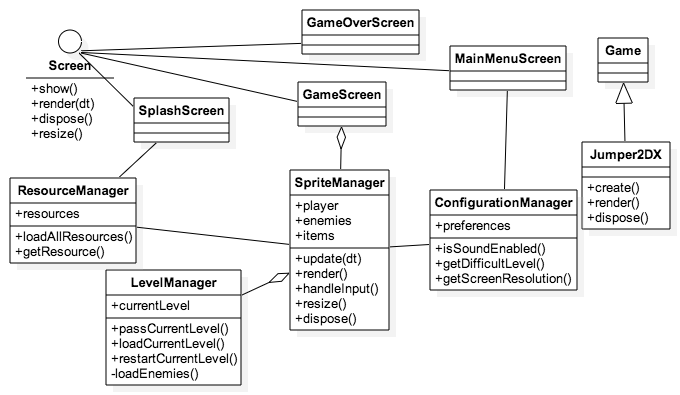
\includegraphics[scale=0.5]{images/uml_game} 
    \caption{Diagrama UML Estados y Managers}
    \end{figure}
\end{frame}


\begin{frame}\frametitle{Proyectos Lanzadera}
	\begin{itemize}
		\item Se crea un proyecto lanzadera para cada plataforma destino del videojuego
		\item Se debe incluir el proyecto principal como dependencia de cada uno de los proyectos lanzadera
		\item En ese proyecto sólo se incluye una clase con un método \emph{main()} que lanza la ejecución del juego
		\item Aunque el proyecto se desarrolle para una única plataforma, incluirá su proyecto lanzadera separado del proyecto principal del videojuego
		\item Debido al funcionamiento de \emph{\textcolor{resalta}{libGDX}}, los \emph{assets} del videojuego se deben incluir en uno de los proyectos lanzadera y enlazarlos desde el resto de proyectos
	\end{itemize}
\end{frame}

\begin{frame}\frametitle{Recursos del videojuego}
    Los recursos son todos aquellos ficheros que no forman parte del código del videojuego. Se localizan dentro de la carpeta
    \emph{\textcolor{resalta}{assets}} en la estructura de alguno de los proyectos lanzadera y se enlazan desde los demás (si los hay)
    \begin{figure}
    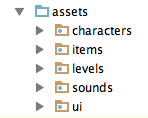
\includegraphics[scale=0.65]{images/assets} 
    \caption{Organización de los assets}
    \end{figure}
\end{frame}

\begin{frame}\frametitle{Empaquetado del videojuego}
    \begin{block}{}
    \begin{itemize}
        \item El empaquetado de la aplicación para su despliegue se hace como el de cualquier otro tipo de aplicación
        \item Se debe hacer del proyecto lanzadera que se quiera desplegar, nunca del proyecto principal
        \item En el caso de proyectos para escritorio, en \emph{IntelliJ} se puede crear un \emph{.jar} desde el menú de \emph{Artefactos}
        \item Para sistemas Windows, utilizando \emph{wrappers} como \textcolor{resalta}{JSmooth}, se pueden crear versiones ejecutables
        \item Para sistemas Android se puede generar el \emph{apk} que corresponda utilizando el proyecto lanzadera de \emph{Android} como si se tratara de una aplicación para dispositivo móvil
    \end{itemize}
    \end{block}
\end{frame}

\section{Hello World!}
\begin{frame}\frametitle{Ejemplo de aplicación}
    \begin{block}{Ejemplo de juego siguiendo la Wiki de \textcolor{resalta}{libGDX}}
    \begin{itemize}
        \item Versión oficial (DropGame v1) \href{https://bitbucket.org/sfaci/java-libgdx/downloads/DropGame_v1.zip}{\beamerbutton{descargar}}
        \item Versión ampliada utilizando \emph{Screens} (DropGame v2)
        \href{https://bitbucket.org/sfaci/java-libgdx/downloads/DropGame_v2.zip}{\beamerbutton{descargar}}
        \item Versión ampliada con más elementos de juego (DropGame v3) \href{https://bitbucket.org/sfaci/java-libgdx/downloads/DropGame_v3.zip}{\beamerbutton{descargar}}
        \item Versión utilizando POO (DropGame POO) \href{https://bitbucket.org/sfaci/java-libgdx/downloads/DropGame_POO.zip}{\beamerbutton{descargar}}
    \end{itemize}
    \end{block}
    Muestra las técnicas básicas en programación de videojuegos: POO, Estados, Managers, Colisiones, HUD y diferentes NPCs
\end{frame}

\section{Componentes libGDX}
\subsection{Componentes UI}
\begin{frame}\frametitle{Elementos de menú}
	\begin{block}{Clases principales}
    \begin{itemize}
        \item \emph{\textcolor{resalta}{Stage}}
        \item \emph{\textcolor{resalta}{Skin}}
		\item \emph{\textcolor{resalta}{Table}} 
		\item \emph{\textcolor{resalta}{Button}} 
		\item \emph{\textcolor{resalta}{CheckBox}} 
		\item \emph{\textcolor{resalta}{Slider}} 
		\item \emph{\textcolor{resalta}{Window}} 
    \end{itemize}
    \end{block}
\end{frame}

\begin{frame}\frametitle{HUD (Head-up display)}
    El \emph{HUD} hace referencia a la información del juego que se muestra al usuario en todo momento. Normalmente serán las vidas
    restantes, la puntuación, algunos objetos que posea el personaje en un momento dado, . . .

    \begin{figure}
    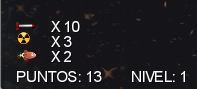
\includegraphics[scale=0.55]{images/hud2}
    \hspace{0.5cm}
    
\includegraphics[scale=0.35]{images/hud1} 
    \caption{HUDs}
    \end{figure}
\end{frame}

\subsection{API 2D}
\begin{frame}\frametitle{API 2D}
	\begin{block}{Sistema de coordenadas en \textcolor{resalta}{libGDX}}
    \begin{figure}
    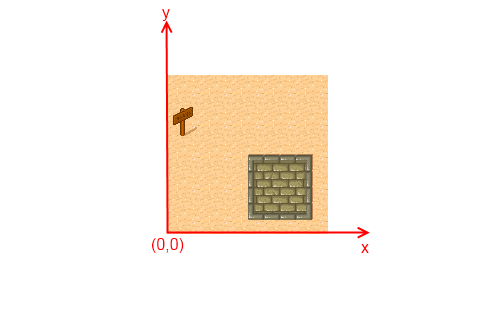
\includegraphics[scale=0.5]{images/xy}
    \caption{Sistema ortogonal (cartesiano)}
    \end{figure}
    \end{block}
\end{frame}

\begin{frame}\frametitle{API 2D}
	\begin{block}{Clases principales}
    \begin{itemize}
        \item \emph{\textcolor{resalta}{Texture}} Representa una imagen en memoria
        \item \emph{\textcolor{resalta}{TextureRegion}} Representa una región delimitada de una textura
        \item \emph{\textcolor{resalta}{Sprite}} Representa una textura con su posición (x,y) en la pantalla
		\item \emph{\textcolor{resalta}{TextureAtlas}} Representa en memoria un mapa de texturas (\emph{texture atlas})
        \item \emph{\textcolor{resalta}{SpriteBatch}} Pinta en pantalla una textura, sprite o frame de animación. También se puede utilizar
        para pintar texto en la pantalla (HUD)
    \end{itemize}
    \end{block}
\end{frame}

\begin{frame}\frametitle{API 2D}
	\begin{block}{Clases principales (continúa)}
    \begin{itemize}
        \item \emph{\textcolor{resalta}{Animation}} Almacena un conjunto de frames (de un sprite) como una animación
        \item \emph{\textcolor{resalta}{Vector2}} Representa la posición \emph{x} e \emph{y} de algún elemento del juego
        \item \emph{\textcolor{resalta}{Rectangle}} Se utiliza para representar el rectángulo de colisión de un elemento del juego. Se
        guarda su posición \emph{x} e \emph{y} y su \emph{anchura} y \emph{altura}
    \end{itemize}
    \end{block}
\end{frame}

\begin{frame}[fragile]\frametitle{Clase Texture}
	\begin{exampleblock}{Texture}
	\begin{lstlisting}[language=java]
// Carga una textura en memoria
Texture texture = new Texture(Gdx.files.internal("items/gun.png"));
// Pinta la textura en una posicion (x, y) determinada de la pantalla
spriteBatch.draw(texture, posicionX, posicionY);
    \end{lstlisting}    
	\end{exampleblock}
\end{frame}

\begin{frame}[fragile]\frametitle{Clase TextureRegion}
	\begin{exampleblock}{TextureRegion}
	\begin{lstlisting}[language=java]
Texture texture = new Texture(Gdx.files.internal("items/weapons.png"));
// "Recorta" una region de la textura indicando x, y, anchura, altura
TextureRegion textureRegion = new TextureRegion(texture, 20, 20, 50, 50);
// Pinta esa zona en pantalla en una posicion (x, y) determinada de la pantalla
spriteBatch.draw(textureRegion, posicionX, posicionY);
    \end{lstlisting}    
	\end{exampleblock}
\end{frame}

\begin{frame}[fragile]\frametitle{Clase Sprite}
	\begin{exampleblock}{Sprite}
    \begin{lstlisting}[language=java]
Texture texture = new Texture(Gdx.files.internal("items/weapons.png"));
// Crea un sprite indicando la region de la textura asignada y su anchura y altura
Sprite sprite = new Sprite(texture, 20, 20, 50, 50);
// Asigna posicion x, y en la pantalla
sprite.setPosition(10, 30);
// Es posible asignar una rotacion al sprite
sprite.setRotation(90);
// Pinta el sprite en pantalla en su posicion
spriteBatch.draw(sprite);
    \end{lstlisting}
	\end{exampleblock}
\end{frame}

\begin{frame}[fragile]\frametitle{Clase TextureAtlas}
	\begin{exampleblock}{TextureAtlas}
    \begin{lstlisting}[language=java]
// Carga el TextureAtlas en memoria
TextureAtlas atlas = new TextureAtlas(Gdx.files.internal("characters/characters.pack"));
// Accede a una textura del atlas por su nombre
Texture texturePlayer = atlas.findRegion("player").getTexture();
// Accede a un grupo de texturas por su nombre
Animation enemyAnimation = new Animation(0.25f, atlas.findRegions("enemy"));
    \end{lstlisting}
	\end{exampleblock}
\end{frame}

\begin{frame}\frametitle{Un texture atlas}
    \begin{figure}
    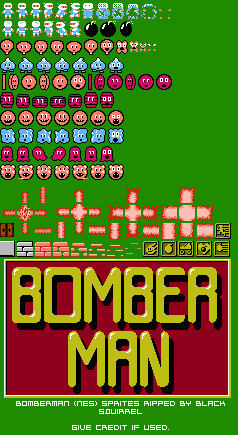
\includegraphics[scale=0.4]{images/textureatlas} 
    \caption{Un texture atlas}
    \end{figure}
\end{frame}

\begin{frame}[fragile]\frametitle{Clase SpriteBatch}
	\begin{exampleblock}{SpriteBatch}
    \begin{lstlisting}[language=java]
spriteBatch.begin();
// Pinta en pantalla los elementos que sea necesario
spriteBatch.draw(personaje, personaje.getX(), personaje.getY());
for (enemigo : enemigos)
    spriteBatch.draw(enemigos, enemigo.getX(), enemigo.getY());
. . .
spriteBatch.end();
    \end{lstlisting}
	\end{exampleblock}
\end{frame}

\begin{frame}\frametitle{Clase Vector2}
    \begin{block}{Vector2}
    \begin{itemize}
        \item \emph{x} Indica el valor de la coordenada x de la posición
        \item \emph{y} Indica el valor de la coordenada y de la posición
        \item \emph{scl(float)} Escala la posición con respecto a un valor (Muy útil para hacerlo con \emph{dt})
        \item \emph{add(Vector2)} Desplaza la posición actual según la posición que se pasa como parámetro
    \end{itemize}
    \end{block}
\end{frame}

\begin{frame}\frametitle{Rectangle}
    Representa el dominio de colisión de un elemento del juego. Es un objeto que no se renderiza, puesto que en su misma posición se
    renderizará la textura o animación del elemento que corresponda. Este objeto sólo lo utilizaremos para calcular colisiones u otro tipo
    de interacción entre dos elementos del juego
    \begin{block}{Rectangle}
    \begin{itemize}
        \item \emph{x} Posición x del rectángulo de colisión
        \item \emph{y} Posición y del rectángulo de colisión
        \item \emph{width} Anchura del rectángulo (normalmente tan ancho como el elemento que representa)
        \item \emph{height} Altura del rectángulo (normalmente tan alto como el elemento que representa)
    \end{itemize}
    \end{block}
\end{frame}

\begin{frame}[fragile]\frametitle{Crear Animaciones}
	El siguiente ejemplo muestra como cargar la animación de un personaje a partir de un \emph{texture atlas}
	\begin{exampleblock}{Ejemplo}
    \begin{lstlisting}[language=java]
// Primero se obtienen los frames con los que queremos crear la animacion
TextureAtlas myAtlas = assetManager.get("my_texture_atlas.pack");
Array<AtlasRegion> allFrames = myAtlas.findRegions("personaje");
. . .
// El primer parametro indica el tiempo entre frames de la animacion, en segundos 
animation = new Animation(0.15f, allFrames);
. . .
// Estas lineas se ejecutaran en los metodos update() y/o render()
stateTime += deltaTime;
TextureRegion currentFrame = animation.getKeyFrame(stateTime, true);
spriteBatch.draw(currentFrame, position.x, position.y);
    \end{lstlisting}
    \end{exampleblock}
    Pincha en el botón para ir al ejemplo \href{https://bitbucket.org/sfaci/libgdx}{\beamerbutton{animaciones}}
\end{frame}

\subsection{Gestión de recursos}
\begin{frame}[fragile]\frametitle{Gestión de recursos}
	La gestión de los recursos del videojuego la realizaremos a través del \emph{AssetManager}, que permite una gestión eficaz de los mismos, a través de nuestro propio \emph{ResourceManager}
	\begin{exampleblock}{ResourceManager}
	\begin{lstlisting}[language=java]
public class ResourceManager implements Disposable, AssetErrorListener {
    . . .
    private AssetManager assetManager;

    public void init() {
        assetManager.setErrorListener(this);
        // Carga el mapa de texturas
        assetManager.load(Constants.A_TEXTURE_ATLAS);
        assetManager.finishLoading();
    }
    . . .
}
	\end{lstlisting}
	\end{exampleblock}
\end{frame}

\begin{frame}{Gestión de recursos (más)}
	\begin{block}{libGDX Texture Packer}
	\begin{itemize}
		\item Aplicación que permite la creación de \emph{texture atlas} a partir de las imágenes
		\item Disponible en \href{https://code.google.com/p/libgdx-texturepacker-gui}{https://code.google.com/p/libgdx-texturepacker-gui}
		\item El fichero resultante (.pack) se carga como recurso del videojuego desde el \emph{ResourceManager}
	\end{itemize}
	\end{block}
\end{frame}

\subsection{Sonido y música}
\begin{frame}[fragile]\frametitle{Sonido y música}
	\begin{block}{Características}
	\begin{itemize}
		\item Formatos soportados: .wav, .mp3, .ogg
		\item Dos interfaces para dar soporte: \emph{Sound} y \emph{Music}
		\item Ambas interfaces incorporan métodos para gestionar el audio: \emph{play(), loop(), stop(), setVolume(float), setLooping(true), isPlaying(), . . .)}
	\end{itemize}
	\end{block}
\end{frame}

\begin{frame}[fragile]{Sonido y música (más)}
	\begin{exampleblock}{Ejemplos}
	\begin{itemize}
		\item \emph{\textcolor{resalta}{Sound}} Pensada para reproducir sonidos cortos
			\begin{lstlisting}[language=java]
Sound sound = Gdx.audio.newSound(Gdx.files.internal("golpe.wav"));
. . .
sound.play();
. . .
sound.dispose();
			\end{lstlisting}
		\item \emph{\textcolor{resalta}{Music}} Pensada para reproducir audios de larga duración
			\begin{lstlisting}[language=java]
Music music = Gdx.audio.newMusic(Gdx.files.internal("cancion.mp3"));
. . .
music.play();
. . .
music.dispose();
			\end{lstlisting}
	\end{itemize}
	\end{exampleblock}
\end{frame}

\subsection{Preferencias}
\begin{frame}[fragile]\frametitle{Preferencias}
	\begin{block}{Guardar / Cargar preferencias (settings)}
	\begin{itemize}
		\item La gestión de las preferencias (settings) de juego del usuario se realiza a través de la clase \emph{Preferences}, que las permite cargar y salvar de forma muy sencilla, abstrayendo al programador del acceso a fichero para realizar esta tarea
		\item El salvado y la carga de preferencias se realizan en nuestro \emph{ResourceManager} a través de la clase \emph{Preferences} que \emph{\textcolor{resalta}{libGDX}} nos proporciona
		\item La clase \emph{Preferences} es la encargada de acceder a fichero y de hacerlo dónde sea conveniente. Nosotros sólo tenemos que indicarle el nombre y valor de la preferencia que queremos guardar/cargar
	\end{itemize}
	\end{block}
\end{frame}

\begin{frame}[fragile]\frametitle{Preferencias (más)}
	\begin{exampleblock}{Ejemplo Preferencias}
	\begin{lstlisting}[language=java]
public class ConfigurationManager {
    public boolean effectSounds;
    public boolean music;
    public int level;
    public float volume;
    private Preferences prefs;
    . . .
    public void load() {
        effectSounds = prefs.getBoolean("effectSounds", true);
        music = prefs.getBoolean("music", true);
        volume = MatUtils.clamp(prefs.getFloat("volume", 0.5f), 0f, 1f);
        level = MathUtils.clamp(prefs.getInteger("startingLevel", 1), 1, 4);
    }

    public void save() {
        prefs.putBoolean("effectSounds", effectSounds);
        prefs.putBoolean("music", music);
        prefs.putFloat("volume", volume);
        prefs.putInteger("startingLevel", level);
    }
}
	\end{lstlisting}
	\end{exampleblock}
\end{frame}

\section{Colisiones}
\begin{frame}[fragile]\frametitle{Colisiones}
    \begin{itemize}
        \item Bounding Box
            \begin{figure}
            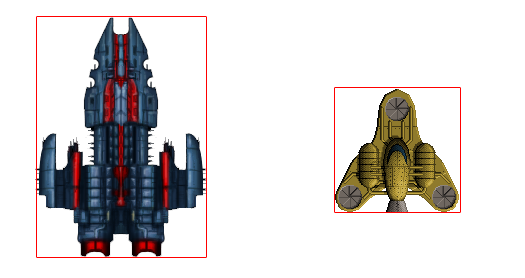
\includegraphics[scale=0.2]{images/collisions1}
            \caption{Colisión Bounding Box}
            \end{figure}
        \item Circle Collision
            \begin{figure}
            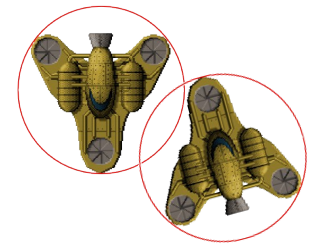
\includegraphics[scale=0.2]{images/collisions2}
            \caption{Colisión Bounding Circle}
            \end{figure}
    \end{itemize}
\end{frame}

\begin{frame}[fragile]\frametitle{Colisiones (II)}
    \begin{itemize}
        \item También podemos combinar los dos anteriores para ajustarnos al tamaño del elemento
            \begin{figure}
            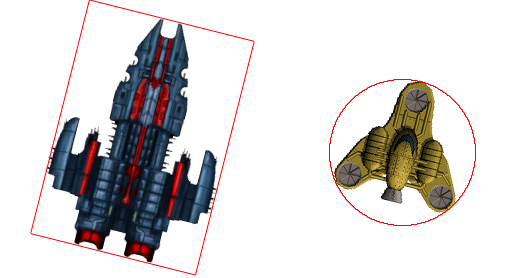
\includegraphics[scale=0.2]{images/collisions3}
            \caption{Bounding Box / Circle}
            \end{figure}
        \item \emph{Bounding circle} y múltiples subdivisiones
            \begin{figure}
            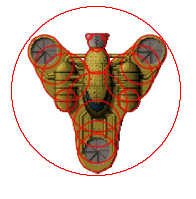
\includegraphics[scale=0.2]{images/collisions4}
            \caption{Múltiples Bounding Circles}
            \end{figure}
    \end{itemize}
\end{frame}

\begin{frame}[fragile]\frametitle{Colisiones (III)}
    \textcolor{resalta}{Rectangle}: Permite definir un \emph{bounding box} con un tamaño y posición determinada y comprobar la
        colisión de éste con otros \emph{Rectangle} utilizando el método \emph{overlaps}
    \begin{exampleblock}{métodos}
    \begin{lstlisting}[language=java]
- float getHeight(), void setHeight(float)
- float getWidth(), void setWidth(float)
- float getX(), void setX(float)
- float getY(), void setY(float)
- void setPosition(Vector2)
- boolean overlaps(Rectangle)
- float perimeter()
. . .
    \end{lstlisting}
    \end{exampleblock}
\end{frame}

\begin{frame}[fragile]\frametitle{Colisiones (IV)}
    \textcolor{resalta}{Circle}: Permite definir un \emph{bounding circle} con un tamaño y posición determinada y comprobar la
        colisión de éste con otros \emph{Circle} utilizando el método \emph{overlaps}
    \begin{exampleblock}{métodos}
    \begin{lstlisting}[language=java]
- float getRadius(), void setRadius(float)
- float getX(), void setX(float)
- float getY(), void setY(float)
- void setPosition(Vector2)
- boolean overlaps(Circle)
- float perimeter()
. . .
    \end{lstlisting}
    \end{exampleblock}
\end{frame}

\begin{frame}[fragile]\frametitle{Colisiones (V)}
    \textcolor{resalta}{Intersector}: Colección de métodos estáticos para detección de colisiones, distancias y otras operaciones
    \begin{exampleblock}{métodos}
    \begin{lstlisting}[language=java]
- overlaps(Circle, Rectangle)
- float distanceLinePoint(float startx, float startY, float endX, float endY, float pointX, float pointY)
- boolean isPointInTriangle(Vector2 point, Vector2 a, Vector2 b, Vector2 c)
. . .
    \end{lstlisting}
    \end{exampleblock}
\end{frame}

\section{Creación de niveles}
\subsection{Tiledmaps}
\begin{frame}\frametitle{¿Qué es un Tiledmap?}
    \begin{itemize}
        \item Un nivel de juego se diseña basándose en baldosas (\emph{tiles}), donde cada baldosa puede representar un elemento diferente
        (tierra, agua, piedra, \ldots)
        \item Una de las formas más sencillas de crear niveles de juego
        \item Se trabaja a partir de kits de baldosas (\emph{tileset}) de donde escoger los diferentes elementos
        \item Posibilidad de incorporar objetos y animaciones a los niveles (enemigos, monedas, items, \ldots)
        \item Tan sencillo como crear un fichero de texto y asignar un carácter a cada tipo de elemento del nivel
    \end{itemize}
\end{frame}

\begin{frame}\frametitle{¿Qué es un Tiledmap? (más)}
    \begin{itemize}
        \item También existe software específico para crear estos mapas \href{http://www.tilededitor.org}{\beamerbutton{tiled}}
        \item Es posible crear mapas de plataformas, de celdas e isómetricos
        \item Se puede trabajar en capas (primer plano, fondo, \ldots)
        \item Muchos frameworks de videojuegos incluyen una \emph{API} específica para trabajar con ellos
        (\emph{\textcolor{resalta}{libGDX}} también)
    \end{itemize}
\end{frame}

\begin{frame}\frametitle{Un Tileset}
    \begin{figure}
    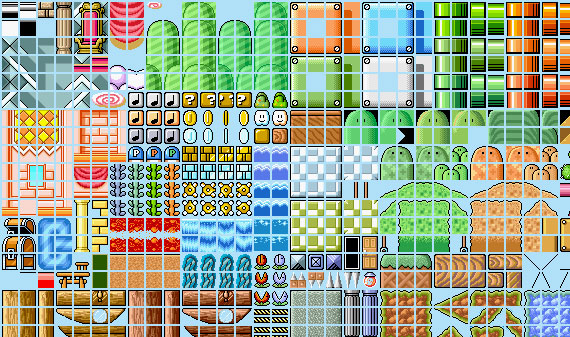
\includegraphics[scale=0.4]{images/tileset}
    \caption{Tileset}
    \end{figure}
\end{frame}

\begin{frame}\frametitle{Un Tiledmap}
    \begin{figure}
    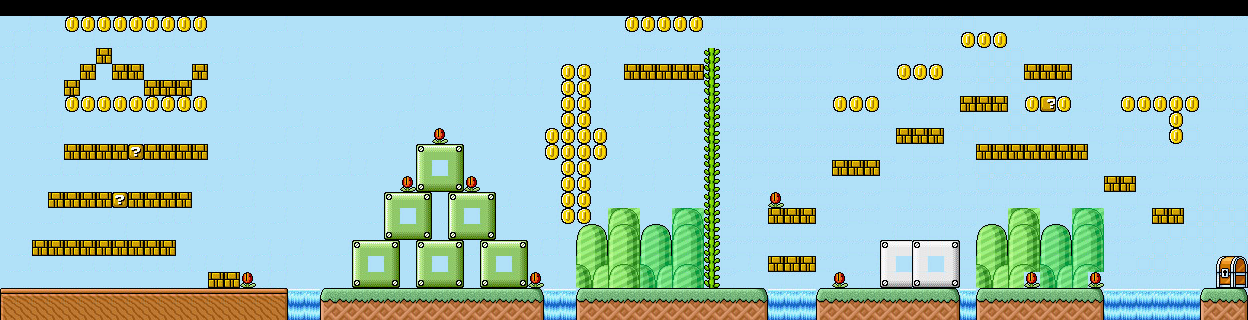
\includegraphics[scale=0.25]{images/tiledmap} 
    \caption{Tilemap (Tiled)}
    \end{figure}
\end{frame}

\begin{frame}\frametitle{Tiled (Editor de mapas)}
    \begin{figure}
    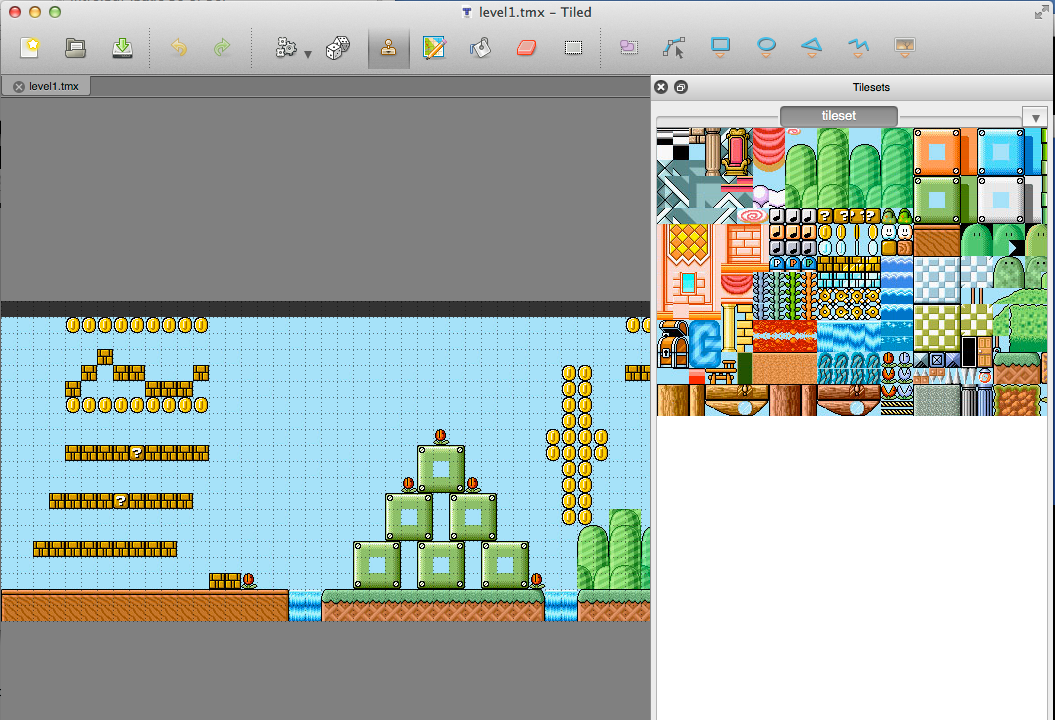
\includegraphics[scale=0.2]{images/tiled} 
    \caption{Tiled (software editor de mapas)}
    \end{figure}
\end{frame}

\begin{frame}\frametitle{Un Tiledmap}
    \begin{figure}
    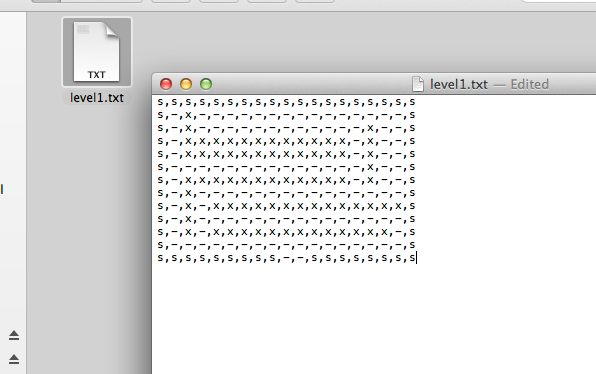
\includegraphics[scale=0.4]{images/tiledmap2} 
    \caption{Tilemap (editor de texto)}
    \end{figure}
\end{frame}

\section{Acceso a Bases de Datos: SQLite}
\begin{frame}\frametitle{¿Qué es SQLite?}
    \begin{block}{Características}
        \begin{itemize}
            \item Motor de Base de Datos de tamaño muy reducido (unos pocos MB)
            \item Ideal para Bases de Datos \emph{pequeñas} (aprox. 1 GB)
            \item No necesita instalación (un único fichero .jar en el caso de Java)
            \item Viene \emph{de serie} con Android
            \item En el desarrollo de videojuegos muy útil para almacenar puntuaciones, partidas, estados de juego, \ldots
            \item Fácil de usar (sólo hay que saber \emph{SQL} y manejarse con \emph{JDBC})
            \item Disponible una \emph{GUI} para \emph{Windows} \href{http://wwww.dondesea.com}{\beamerbutton{sqliteadmin}}
        \end{itemize}
    \end{block}
\end{frame}

\begin{frame}[fragile]\frametitle{¿Cómo funciona SQLite en libGDX?}
    Al tratarse de un único fichero .jar, se añade como librería del proyecto, se carga el driver JDBC y se trabaja directamente con SQL
    como con cualquier otro \emph{SGBD}
    \begin{exampleblock}{Conexión con SQLite}
    \begin{lstlisting}[language=java]
Class.forName("org.sqlite.JDBC");		

Connection connection = null;
connection = DriverManager.getConnection("jdbc:sqlite:" + Gdx.files.internal("scores.db"));	

Statement statement = connection.createStatement();
statement.executeUpdate("CREATE TABLE IF NOT EXISTS scores (id integer primary key autoincrement, name text, score int)");
statement.executeUpdate("INSERT INTO scores (name, score) VALUES ('" + name + "', " + score + ")");
	
// Cerrar statement y connection
// Capturar excepciones
    \end{lstlisting}
    \end{exampleblock}
\end{frame}

\begin{frame}\frametitle{Proyectos de Ejemplo}
    \begin{itemize}
        \item Estructura de un proyecto libGDX \href{https://bitbucket.org/sfaci/java-libgdx/downloads/EstructuraProyectoLibgdx.zip}{\beamerbutton{descargar}}
        \item Juego Simple I (DropGame) \href{https://bitbucket.org/sfaci/libgdx/downloads/DropGame_v1.zip}{\beamerbutton{descargar}}
        \item Juego Simple II (DropGame) \href{https://bitbucket.org/sfaci/libgdx/downloads/DropGame_v2.zip}{\beamerbutton{descargar}}
        \item Juego Simple III (DropGame) \href{https://bitbucket.org/sfaci/libgdx/downloads/DropGame_v3.zip}{\beamerbutton{descargar}}
        \item Juego Simple POO (DropGame) \href{https://bitbucket.org/sfaci/libgdx/downloads/DropGame_POO.zip}{\beamerbutton{descargar}}
        \item Trabajar con animaciones I \href{https://bitbucket.org/sfaci/libgdx/downloads/animaciones.zip}{\beamerbutton{descargar}}
        \item Juego de plataformas (Jumper2dx) \href{https://bitbucket.org/sfaci/jumper2dx/downloads/jumper2dx-desktop_v0.2.jar}{\beamerbutton{descargar}}
        \item Juego de plataformas (minijumper2dx) \href{https://bitbucket.org/sfaci/minijumper2dx}{\beamerbutton{acceder}}
        \item Juego de naves (JFighter2dx) \href{https://bitbucket.org/sfaci/jfighter2dx/downloads/jfighter2dx-desktop_v1.jar}{\beamerbutton{descargar}}
        \item Juego de mapas (bombermanx) \href{https://bitbucket.org/sfaci/jbombermanx/downloads/jbombermanx_v0.1.jar}{\beamerbutton{descargar}}
        \item Juego tipo RPG (Robin2dx) \href{https://bitbucket.org/sfaci/java-libgdx/downloads/robin2dx.zip}{\beamerbutton{descargar}}
        \item Juego tipo puzzle (Arkanoidx) \href{https://bitbucket.org/sfaci/arkanoidx/downloads/arkanoidx-desktop_v0.1.jar}{\beamerbutton{descargar}}
    \end{itemize}
\end{frame}

\begin{frame}\frametitle{Más información}
    \begin{itemize}
        \item Repositorio de los proyectos en \emph{Bitbucket} \href{https://bitbucket.org/sfaci/java-libgdx}{\beamerbutton{acceder}}
        \item Página Web de \emph{\textcolor{resalta}{libGDX}} \href{https://libgdx.badlogicgames.com}{\beamerbutton{acceder}}
        \item Wiki de \emph{\textcolor{resalta}{libGDX}} \href{https://github.com/libgdx/libgdx/wiki}{\beamerbutton{acceder}}
        \item Javadoc de \emph{\textcolor{resalta}{libGDX}} \href{https://libgdx.badlogicgames.com/nightlies/docs/api}{\beamerbutton{acceder}}
        \item Videotutoriales sobre \emph{\textcolor{resalta}{libGDX}} en \href{http://videosdeinformatica.com}{videosdeinformatica.com}
        \href{https://videosdeinformatica.com/tag/libgdx}{\beamerbutton{acceder}}
    \end{itemize}
\end{frame}

\end{document}
